% generated by make_figs.mjs
\resizebox{\columnwidth}{!}{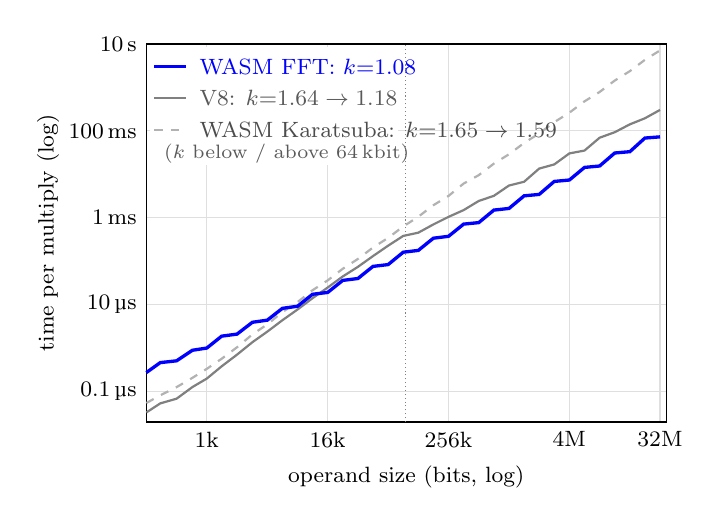
\begin{tikzpicture}[font=\footnotesize]
\draw[gray!25] (0,0.386) -- (6.6,0.386); \node[left] at (0,0.386) {0.1\,\textmu s};
\draw[gray!25] (0,1.490) -- (6.6,1.490); \node[left] at (0,1.490) {10\,\textmu s};
\draw[gray!25] (0,2.593) -- (6.6,2.593); \node[left] at (0,2.593) {1\,ms};
\draw[gray!25] (0,3.697) -- (6.6,3.697); \node[left] at (0,3.697) {100\,ms};
\draw[gray!25] (0,4.800) -- (6.6,4.800); \node[left] at (0,4.800) {10\,s};
\draw[gray!25] (0.767,0) -- (0.767,4.8); \node[below] at (0.767,0) {1k};
\draw[gray!25] (2.302,0) -- (2.302,4.8); \node[below] at (2.302,0) {16k};
\draw[gray!25] (3.837,0) -- (3.837,4.8); \node[below] at (3.837,0) {256k};
\draw[gray!25] (5.372,0) -- (5.372,4.8); \node[below] at (5.372,0) {4M};
\draw[gray!25] (6.523,0) -- (6.523,4.8); \node[below] at (6.523,0) {32M};
\draw (0,0) rectangle (6.6,4.8);
\node at (3.3,-0.7) {operand size (bits, log)};
\node[rotate=90] at (-1.25,2.4) {time per multiply (log)};
\draw[gray,densely dotted] (3.294,0) -- (3.294,4.8) node[below left,align=right,font=\scriptsize] {V8 switches\\to its FFT};
\draw[gray,thick] plot coordinates {(0.000,0.121) (0.176,0.236) (0.384,0.296) (0.585,0.444) (0.767,0.551) (0.956,0.707) (1.151,0.855) (1.346,1.013) (1.535,1.147) (1.727,1.292) (1.919,1.428) (2.110,1.572) (2.302,1.707) (2.494,1.848) (2.686,1.970) (2.878,2.107) (3.070,2.239) (3.262,2.363) (3.453,2.404) (3.645,2.509) (3.837,2.605) (4.029,2.691) (4.221,2.807) (4.413,2.872) (4.605,3.003) (4.797,3.051) (4.988,3.218) (5.180,3.271) (5.372,3.411) (5.564,3.447) (5.756,3.610) (5.948,3.680) (6.140,3.780) (6.331,3.857) (6.523,3.963)};
\draw[gray!60,thick,dashed] plot coordinates {(0.000,0.241) (0.176,0.338) (0.384,0.443) (0.585,0.561) (0.767,0.675) (0.956,0.803) (1.151,0.949) (1.346,1.112) (1.535,1.239) (1.727,1.396) (1.919,1.522) (2.110,1.673) (2.302,1.798) (2.494,1.946) (2.686,2.070) (2.878,2.216) (3.070,2.338) (3.262,2.483) (3.453,2.606) (3.645,2.753) (3.837,2.871) (4.029,3.028) (4.221,3.135) (4.413,3.281) (4.605,3.400) (4.797,3.544) (4.988,3.664) (5.180,3.808) (5.372,3.928) (5.564,4.072) (5.756,4.191) (5.948,4.336) (6.140,4.456) (6.331,4.599) (6.523,4.719)};
\draw[blue,very thick] plot coordinates {(0.000,0.628) (0.176,0.754) (0.384,0.777) (0.585,0.911) (0.767,0.939) (0.956,1.090) (1.151,1.116) (1.346,1.266) (1.535,1.293) (1.727,1.443) (1.919,1.470) (2.110,1.622) (2.302,1.645) (2.494,1.798) (2.686,1.822) (2.878,1.976) (3.070,1.999) (3.262,2.156) (3.453,2.179) (3.645,2.334) (3.837,2.358) (4.029,2.513) (4.221,2.532) (4.413,2.691) (4.605,2.712) (4.797,2.872) (4.988,2.890) (5.180,3.055) (5.372,3.073) (5.564,3.233) (5.756,3.251) (5.948,3.416) (6.140,3.433) (6.331,3.606) (6.523,3.621)};
\fill[white] (0.051,3.262) rectangle (3.201,4.762);
\draw[blue,very thick] (0.101,4.512) -- +(0.4,0);
\node[blue,anchor=west] at (0.551,4.512) {WASM FFT: $k{=}1.08$};
\draw[gray,thick] (0.101,4.112) -- +(0.4,0);
\node[gray!70!black,anchor=west] at (0.551,4.112) {V8: $k{=}1.64 \to 1.18$};
\draw[gray!60,thick,dashed] (0.101,3.712) -- +(0.4,0);
\node[gray!60!black,anchor=west] at (0.551,3.712) {WASM Karatsuba: $k{=}1.65 \to 1.59$};
\node[anchor=west,font=\scriptsize,gray!70!black] at (0.101,3.412) {($k$ below / above 64\,kbit)};
\end{tikzpicture}}
